\documentclass[11pt,letterpaper]{article}
\usepackage[margin=0.75in]{geometry}
\usepackage[T1]{fontenc}
\usepackage{lmodern}
\usepackage{amsmath,amssymb}
\usepackage{graphicx}
\usepackage{booktabs}
\IfFileExists{placeins.sty}{\usepackage{placeins}}{}
\usepackage{float}
\IfFileExists{balance.sty}{\usepackage{balance}}{}
\usepackage{setspace}
\setstretch{1.12}
\raggedbottom
\usepackage[numbers,sort&compress]{natbib}
\usepackage[bookmarks=false]{hyperref}
\usepackage[font=small,labelfont=bf]{caption}
\usepackage{xcolor}
% Text added or changed since the previous version.
\definecolor{darkred}{HTML}{8B0000}
\newcommand{\new}[1]{\textcolor{darkred}{#1}}

\graphicspath{{figures/}{./}}
\makeatletter\def\input@path{{figures/}{./}}\makeatother % lets \IfFileExists find the figure files too

% ---------------------------------------------------------------------------
% Figure files, one macro each, path without extension. Repoint a figure here
% and every use follows. The stored file names do not match the printed figure
% numbers, so the number each macro produces is noted beside it.
% ---------------------------------------------------------------------------
\newcommand{\figworkflow}{workflow}                      % Figure 1 (unused; fig1.pdf is included directly)
\newcommand{\figperformance}{fig2_prediction_transfer}   % Figure 2
\newcommand{\figexternal}{fig3_external_validation}      % Figure 3
\newcommand{\figcontext}{fig4_context_mechanism}         % Figure 4
\newcommand{\figcandidates}{fig5_variant_prioritization} % Figure 5

\setlength{\columnsep}{0.30in}
\setlength{\parskip}{0.35em}
\setlength{\parindent}{1em}
\renewcommand{\arraystretch}{1.03}
\setlength{\textfloatsep}{15pt plus 3pt minus 3pt}
\setlength{\floatsep}{12pt plus 3pt minus 2pt}
\setlength{\intextsep}{12pt plus 3pt minus 2pt}
\setlength{\emergencystretch}{1.5em}
\renewcommand{\topfraction}{0.92}
\renewcommand{\bottomfraction}{0.70}
\renewcommand{\textfraction}{0.06}
\renewcommand{\floatpagefraction}{0.75}
\setcounter{topnumber}{2}
\setcounter{totalnumber}{3}

\setcounter{topnumber}{4}
\setcounter{bottomnumber}{2}
\setcounter{totalnumber}{6}
\renewcommand{\topfraction}{0.95}
\renewcommand{\bottomfraction}{0.85}
\renewcommand{\textfraction}{0.05}
\renewcommand{\floatpagefraction}{0.80}
\setcounter{dbltopnumber}{2}
\renewcommand{\dbltopfraction}{0.95}
\renewcommand{\dblfloatpagefraction}{0.80}

\renewenvironment{abstract}{%
  \section*{\abstractname}\vspace{-0.25em}
}{\par\vspace{0.6em}}

\hypersetup{colorlinks=true, linkcolor=black, citecolor=black, urlcolor=black}


\newcommand{\added}[1]{#1}
\usepackage{tikz}
\usetikzlibrary{arrows.meta,positioning}
\definecolor{seqblue}{HTML}{135E96}
\definecolor{ctxgreen}{HTML}{239DAD}
\definecolor{fusionpurple}{HTML}{168BC4}
\newcommand{\figureplan}[2]{\fbox{\parbox[c][42mm][c]{0.93\linewidth}{\centering\small
\textbf{Figure assembly pending: #1}\\[4pt]#2\\[4pt]
\footnotesize Panel specifications and source paths: FIGURE\_GUIDE.md}}}

\title{\LARGE\bfseries SilentMethyl: a multimodal framework for CpG methylation prediction and local variant-effect inference}
\author{%
  Samuel Zhang$^{1,2}$, Shaojun Pei$^{1,2,*}$, and Gil Alterovitz$^{1,2,*}$ \\[0.5em]
  \small $^{1}$Division of General Internal Medicine and Primary Care, \\
  \small Brigham and Women's Hospital, Boston, Massachusetts, United States \\
  \small $^{2}$Harvard Medical School, Harvard University, Boston, Massachusetts, United States \\[0.5em]
  \small $^{*}$Authors for correspondence: \href{mailto:spei1@bwh.harvard.edu}{spei1@bwh.harvard.edu} (Shaojun Pei); \\
  \small \href{mailto:gil\_alterovitz@hms.harvard.edu}{gil\_alterovitz@hms.harvard.edu} (Gil Alterovitz)
}
\renewcommand{\thepage}{\arabic{page}}
\date{}


\begin{document}
\maketitle
\begin{abstract}
Predicting how nucleotide variants influence local methylation remains challenging. We developed SilentMethyl, a multimodal framework integrating DNA sequence with epigenomic context to predict methylation and infer local variant effects. SilentMethyl achieved a beta-value MAE of 0.0914 and ROC-AUC of 0.9744 across 26,570 held-out CpGs, outperforming sequence-only and context-only models as well as retrained CpGenie and DeepCpG. Context reduced prediction error by 22.4\% and 22.9\% at CpGs with high ATAC-seq or H3K27ac signal, respectively. Cross-tissue predictions were most accurate at CpGs with low methylation variability across tissues. Predicted effects showed modest concordance with independent mQTL and allele-specific methylation data, with signed Spearman correlations of 0.236 in eGTEx breast and 0.149 in GENOA blood. Variant-CpG distance contributed substantially to apparent discrimination of mQTL-associated variants, with fusion AUROC decreasing from 0.600 to 0.556 after distance matching. Context influenced variant predictions, but fusion did not clearly outperform sequence-only on external validation benchmarks. SilentMethyl also predicted a local methylation change around a pathogenic STK11 stop-gain variant and independently prioritized a synonymous NCOA2 variant among 440 held-out TCGA-BRCA SNV-CpG pairs. Overall, SilentMethyl provides a multimodal framework for accurate CpG methylation prediction and inference of local variant effects, enabling variant prioritization for targeted experimental validation.
\end{abstract}

\section{Introduction}
DNA methylation is a major component of epigenetic regulation and is closely associated with genomic context, chromatin organization, and transcriptional activity \cite{jones2012functions,schubeler2015function}. Single-nucleotide variants (SNVs) can also be associated with local differences in DNA methylation, providing a potential link between genetic variation and epigenetic regulation. However, directly characterizing the methylation consequences of individual variants remains challenging because datasets containing matched genetic and epigenetic measurements are limited, while experimental testing of large numbers of candidate variants is difficult. Computational models that predict CpG methylation from genomic information may therefore provide a useful means of identifying loci and variants for downstream functional investigation.

Deep learning approaches have shown that DNA sequence contains substantial information for predicting methylation and other regulatory properties \cite{angermueller2017deepcpg,zhou2015predicting,avsec2021effective,camillo2024cpgpt}. Existing methylation-prediction frameworks use different combinations of local sequence, neighboring methylation measurements, tissue information, and epigenomic features. CpGenie predicts CpG methylation from local DNA sequence and evaluates sequence substitutions using methylation quantitative trait loci (mQTLs) \cite{zeng2017cpgenie}, whereas other approaches incorporate tissue-specific or chromatin information, including INTERACT, DeepMethylation, Methven, and more recent multi-cell-type methylation models \cite{zhou2022interact,li2026deepmethylation,liu2025methven,jin2026melody}. Together, these studies indicate that both DNA sequence and the surrounding regulatory environment can contribute to methylation prediction.

However, predicting the methylation state of a genomic locus and predicting the change in methylation caused by a nucleotide substitution are related but distinct problems. A model can predict baseline methylation accurately without necessarily predicting a local variant effect with comparable accuracy. This distinction is particularly important when reference epigenomic features are incorporated into the model. Chromatin accessibility, histone modifications, and evolutionary conservation may provide useful information about the methylation state at a CpG locus, whereas paired REF and ALT sequences are evaluated at the same genomic locus and therefore share the same reference epigenomic context. Context can still influence how a sequence change is interpreted by the model, but improved prediction of baseline methylation does not necessarily imply improved prediction of the allelic difference. Baseline methylation prediction and variant-effect prediction should therefore be evaluated separately.

A separate challenge is how variant-effect predictions should be evaluated. Because substitutions are scored within a CpG-centered sequence window, predicted effects can depend not only on the nucleotide change and its local sequence environment, but also on the position of the variant relative to the target CpG. Experimentally associated variant--CpG pairs may likewise differ systematically in distance from control pairs. As a result, apparent discrimination of methylation-associated variants can partly reflect distance-related positional information. Controlling for variant--CpG distance is therefore important when assessing whether predicted effect magnitudes preferentially identify associated variants.

To address these questions, we developed SilentMethyl, a multimodal framework for predicting CpG methylation and local variant effects by integrating DNA sequence with reference epigenomic context. SilentMethyl was designed to evaluate these two tasks separately. Baseline methylation performance was assessed on chromosome-level held-out CpGs, whereas variant-effect predictions were compared with independent mQTL association estimates and allele-specific methylation data as external evidence of allele-associated methylation differences. We further evaluated whether predicted effect magnitudes could distinguish associated from control variant--CpG pairs before and after controlling for variant--CpG distance, and examined how reference epigenomic context influenced predicted variant effects.

SilentMethyl achieved accurate baseline methylation prediction on 26,570 held-out CpGs, with a beta-value MAE of 0.0914 and ROC-AUC of 0.9744, outperforming the sequence-only and context-only models as well as CpGenie and DeepCpG retrained on the same data splits. Incorporating epigenomic context consistently improved baseline methylation prediction, although the magnitude of improvement varied across regulatory environments. In contrast, prediction of local variant effects was substantially more challenging. Predicted effects showed modest concordance with independent mQTL association estimates and allele-specific methylation data, and discrimination of mQTL-associated variants was reduced after matching for variant--CpG distance. Although epigenomic context influenced the predicted variant effects, the fusion model did not clearly outperform the sequence-only model on these external benchmarks. Together, these findings highlight the distinction between predicting methylation state and predicting methylation changes associated with nucleotide variation, and support the use of SilentMethyl as a prioritization tool for identifying variants with potential local methylation effects for targeted downstream functional validation.

\section{Methods}
\subsection{Data construction}
Methylation beta labels were constructed from the TCGA-BRCA HM450 matrix \cite{tcga2012breast,grossman2016gdc}. Using a sample-type-11 filter, 97 solid-tissue-normal columns were selected from 893 total. We checked that these 97 columns represented 97 unique participants without duplicate samples.

We represented single-probe methylation as the median of patient beta values. For CpG $i$, if $O_i$ represents the set of patients with a recorded methylation measurement at CpG $i$, then
\begin{gather*}
\beta_i=\operatorname{median}_{s\in O_i}\beta_{i,s},
\qquad y_i=\mathbf{1}[\beta_i>0.5],\\
\widetilde\beta_i=\max\left(10^{-4},\min\left(1-10^{-4},\beta_i\right)\right),\\
M_i=\log_2\left(\frac{\widetilde\beta_i}{1-\widetilde\beta_i}\right).
\end{gather*}
The transformation from beta to $M$-values follows \cite{du2010betamvalue}. 

All probes required an exact CpG centered DNA sequence and a valid reference context window. None of the 418,486 probes in our combined dataset were flagged by HM450's \texttt{MASK\_general} filter. Median CpG probe coverage in our dataset was 97 out of 97 total, and 95.1\% of loci had at least 78 valid patients (Supplementary Fig.~S1). Probe coordinates and DNA sequence were then pulled from the hg38 HM450 annotation resource \cite{zhou2017infinium,chen2013crossreactive}.

The data was split by chromosome into training, validation, and test sets before model training. Chromosomes 10--11 formed the validation set, chromosomes 8--9 formed the test set, and the remaining chromosomes formed the training set. The corresponding locus counts were 345,359, 46,557 and 26,570. By separating data by chromosome, we ensured no sequence windows overlapped between training, validation, and testing sets. We performed three additional single-seed evaluations on test chromosomes 12/18, 4/20 and 13/15/21. 

Each DNA input comprised a 1,000-bp CpG-centered sequence. The target CpG nucleotides were located at 499 and 500(zero-indexed). The epigenetic input comprised of seven breast-epithelium attributes, including ATAC-seq chromatin accessibility and six histone marks(H3K4me3, H3K27ac, H3K27me3, H3K9me3, H3K36me3, H3K4me1), averaged across a CpG centered 100 bp sequence. Breast context also contained two PhyloP scores for the two nucleotides in the center CpG \cite{pollard2010phylop}. A missingness mask was assigned to each feature. Missing values were imputed using the corresponding feature's global median. The reference data were derived from shared resources and were not patient-specific.

\subsection{Models and staged training}
The sequence module comprised a pretrained DNABERT-2 (117M) transformer \cite{zhou2024dnabert2}, followed by a convolutional layer. Masked attention pooling was then applied:
\[
\alpha_t=\frac{\exp(s_t)}{\sum_{u\in V}\exp(s_u)},\qquad
\mathbf h_{\rm seq}=\sum_{t\in V}\alpha_t\mathbf e_t,
\]
where $V$ contains non-padding positions and $\mathbf e_t$ denotes the embedding at position $t$. This produced a 768-dimensional sequence representation. The context component consisted of an MLP mapping the 18-dimensional reference input (nine features and nine masks) to a second 768-dimensional vector, $\mathbf h_{\rm ctx}$.

After LayerNorm, the two embeddings were concatenated into a 1,536-dimensional vector and passed through a gating MLP that produced $g_{\rm seq}$ and $g_{\rm ctx}$. The fused embedding was
\[
\mathbf z=g_{\rm seq}\widetilde{\mathbf h}_{\rm seq}
+g_{\rm ctx}\widetilde{\mathbf h}_{\rm ctx}.
\]
Two prediction heads used this embedding. The regression head predicted $M$, converted to beta by $\widehat\beta=2^{\widehat M}/(1+2^{\widehat M})$. The classification head produced a methylation probability, with the binary call defined by a threshold of 0.5. The training objective was the sum of Huber loss ($\delta=1.345$) on regression and binary cross-entropy on classification. 

Sequence and context models were trained independently with AdamW\cite{loshchilov2019adamw}, with DNABERT-2 fully fine-tuned. Sequence, context, and fusion training used up to 10, 15, and 10 epochs and learning rates of $2\times10^{-5}$, $10^{-3}$, and $5\times10^{-4}$, respectively. During fusion training, the component models were frozen and only the normalization, gating, and prediction modules were updated. Forward or reverse-complement DNA orientation was chosen with equal probability for each probe. For each model seed of 42, 43, and 44, the checkpoint model was chosen by lowest validation beta MAE. 

Primary prediction metrics included RMSE and MAE for both $\beta$ and $M$ values for regression, and ROC-AUC for classification. We also rebuilt CpGenie and DeepCpG's DNA module and trained them on the same settings as our models. In addition, we included composition and reverse-complement-collapsed $k$-mer ridge models as simpler sequence baselines.

\subsection{Paired scoring and synonymous variant construction}
For each SNV, predicted methylation difference was calculated and averaged across forward and reverse complement strands: 
\begin{align*}
\Delta\widehat\beta=\tfrac12\big[&\widehat\beta_{\mathrm{ALT,FWD}}-\widehat\beta_{\mathrm{REF,FWD}}\\
+&\widehat\beta_{\mathrm{ALT,RC}}-\widehat\beta_{\mathrm{REF,RC}}\big].
\end{align*}
$\Delta\widehat M$ was defined similarly. The reference context was held fixed between alleles. 

Tagged somatic sSNVs were obtained through the GDC and amino acid preservation was verified through hg38 and GENCODE v44 \cite{grossman2016gdc,frankish2021gencode}. Variants were then matched with the closest existing HM450 CpG probe. 440 unique variants remained after filtering out variants with probes flagged by \texttt{MASK\_general} and outside the 1000 bp window of their CpG.
Variants were prioritized by $|\Delta\widehat\beta|$, predicted from the seed-42 model. For each variant, we recorded FWD-RC prediction difference, and relative rank against other synonymous variants with similar mutation context and distance to CpG. Nonsynonymous examples were processed through the same scoring procedure as well. 

\subsection{External mQTL evaluation}
We converted GENOA coordinates \cite{shang2023genoa} from hg19 to hg38 and checked that REF alleles matched the reference genome. We also adjusted reported effect signs to match the model's REF-to-ALT direction. After ensuring that all variants fell in the target probe sequence window, we were left with 66,495 held-out pairs. Removing variants that created or destroyed a CpG left 42,866 pairs, including 4,037 significant ones at $p<5\times10^{-8}$. In eGTEx breast \cite{oliva2023mqtl}, 76,893 pairs remained after sequence window filtering, including 418 significant pairs that did not create or destroy a CpG. We used a significance cutoff of $1.483\times10^{-5}$. 

Signed Spearman correlation compared predicted and measured effect rankings. Directional agreement and AUROC evaluated how often difference signs matched, and whether predictions separated positive from negative measured effects, respectively. Absolute predicted and measured effects were also correlated to compare magnitude rankings. Discrimination AUROC tested if the magnitude of predicted differences separated significant from nonsignificant pairs. We also matched variants by variant--CpG distance within 10 bp and compared models on these pairs. Distance-only AUROC checked if distance still separated these matched groups.

A smaller positive-control analysis used significant eGTEx breast lead mQTLs ($q<0.05$) at held-out CpGs. Filtering out CpG-destructive variants left 81 associations from 70 unique variants. We also repeated the analysis without variants on or directly adjacent to their probe. For a separate comparison, we matched significant and nonsignificant lead variants ($q\geq0.5$) on chromosome and minor allele frequency, allowing a frequency difference of at most 0.05. We matched mQTLs by similar distance, baseline methylation and base-change type. This produced 35 matched pairs from 53 significant and 51 nonsignificant variants. We resampled matched pairs for confidence intervals and randomly swapped labels within each pair to test discrimination against random chance.

\subsection{Allele-specific methylation evaluation}
We used allele-specific methylation (ASM) data from the Rosenski--Dor--Kaplan \cite{rosenski2025asm} and Do--Tycko \cite{do2020asm} cohorts. We only included variants on held-out chromosomes and within the 1,000-bp CpG-centered DNA sequence. For Do--Tycko, predicted $\Delta\widehat M$ was averaged across scored CpGs in each index SNP's differentially methylated region (DMR), giving 722 SNP-level comparisons. Predicted differences were evaluated using direction agreement, signed Spearman correlation and directional AUROC, which measures how well signed predictions separate positive from negative measured effects. These tests all used a fixed model seed of 42. 

We built control datasets to test if predicted effects separated ASM from controls for each cohort. Rosenski controls were loci with bimodal methylation but no ASM, while Do--Tycko controls were loci outside DMRs. Both were matched by variant--CpG distance. These test sets contained 6,910 and 10,746 variant--CpG pairs, respectively. Confidence intervals were constructed based on resampled 1Mb blocks, using 179 blocks for the Do--Tycko signed analysis and 242 for the Rosenski discrimination analysis. The additional restriction of $|\Delta\beta_{\mathrm{observed}}|\geq0.2$ was applied after the initial analysis. Detailed sampling procedures and confidence intervals for each model are provided in Supplementary Table~S2.

\subsection{Transfer and gate decomposition}
For multi-tissue training, we assigned each probe to one tissue so that a fixed DNA sequence was not assigned different methylation targets from multiple tissues. Colon, kidney and lung targets were built from TCGA HM450 solid-tissue-normal samples (TCGA-COAD, 38; TCGA-KIRC, 160; TCGA-LUAD and TCGA-LUSC, 74), using the same context features from tissue-matched ENCODE tracks. Training probes were drawn from probes covered in every tissue and randomly assigned in equal numbers (115,119 per tissue). The breast-held-out model excluded breast data from training and validation and was evaluated on the same breast test CpGs as the breast-trained model. We compared prediction error with measured cross-tissue methylation variance, both before and after controlling for mean methylation. The breast-held-out model used one training seed and was compared with the three-seed breast-only mean. 

To examine how sequence and gate changes contributed to each predicted variant effect, we changed them one at a time. Let $H$ be the trained regression head, $d_R$ and $d_A$ the normalized REF and ALT sequence representations, and $c$ the fixed normalized context representation. The weights $g_d$ and $g_c$ are the sequence and context gate weights, with $R$ and $A$ indicating the allele used to calculate them. We constructed four representations:

\begin{align*} z_R&=g_{d,R}d_R+g_{c,R}c,\\ z_S&=g_{d,R}d_A+g_{c,R}c,\\ z_D&=g_{d,A}d_A+g_{c,R}c,\\ z_A&=g_{d,A}d_A+g_{c,A}c. \end{align*}

Starting from the REF representation $z_R$, we first replaced the sequence representation with its ALT value to obtain $z_S$, then replaced the sequence-gate weight to obtain $z_D$, and finally the context-gate weight to obtain the full ALT representation $z_A$. The prediction changes $H(z_S)-H(z_R)$, $H(z_D)-H(z_S)$ and $H(z_A)-H(z_D)$ define the sequence, sequence-gate and context-gate components. These changes sum to the full predicted variant effect. The last two components together form the combined gate contribution.

We calculated fusion components separately for forward and reverse-complement orientations and then averaged them. Partial rank correlations measured the relationship between gate contributions and observed effects after controlling for the sequence component. We also compared predictions using unchanged context, context shuffled between probes and context replaced with feature medians. For each prediction type, we divided the mean absolute change by the standard deviation of the original predictions, so changes in baseline methylation and variant effects can be compared on a common scale. 

\subsection{Statistical analysis and interpretation controls}
We calculated confidence intervals by repeatedly resampling  1-Mb genomic blocks to keep nearby observations together. Paired comparisons of baseline methylation models used 5,000 sampling repeats. Analyses on primary external cohorts and ASM used 2,000 repeats, cross-cohort analyses used 500, and gate analyses used 1,000. Stratified fusion gains and uncertainty correlations used 2,000, transfer-error intervals used 400, and comparisons with retrained published models on external cohorts, motif analyses and GWAS analyses used 500. Standard deviations across training seeds were reported separately from block sampling intervals, since they measure different sources of variation. Additional chromosome splits were trained and evaluated separately. 

After model evaluation, we grouped held-out probes by GENCODE region, position relative to CpG islands and chromatin-signal quartiles. We calculated absolute improvement in each group as sequence-only $\beta$ MAE minus fusion $\beta$ MAE. Relative improvement was this difference over sequence-only $\beta$ MAE.

We tested whether disagreement between forward and reverse-complement predictions could identify less reliable predictions. We compared this measure with prediction variability across training seeds, a score measuring closeness to $\widehat\beta=0.5$ ($-|\widehat\beta-0.5|$), and a random control. We measured how each score correlated with prediction error. We also tested how average error changed as predictions with higher uncertainty scores were removed. These analyses were done on both the $\beta$ and $M$ scales, and within groups of similar predicted $\beta$ values.

We also identified JASPAR motifs on both DNA strands \cite{rauluseviciute2024jaspar}. For each motif, we found the highest scoring WT match and scored the MUT sequence at the same position and orientation. We then tested if changes in motif scores were related to predicted methylation effects, while controlling for sequence composition, variant--CpG distance and the type of base change. We also adjusted for the increased chance of false positives when testing many motifs.

We identified GWAS-listed variants \cite{cerezo2025gwas} by rsID or genomic coordinate among held-out variant--CpG pairs with measured mQTL $p<0.05$. We matched listed and unlisted variants by variant--CpG distance and allele frequency, then tested if listed variants were more common among pairs with larger predicted difference magnitudes. Confidence intervals were calculated by resampling genomic blocks. More details and source data are provided in the Supplementary data.


\section{Results}
\subsection{Multimodal fusion accurately predicts baseline CpG methylation}
\label{sec:performance}
SilentMethyl's fusion model combines a 1,000-bp CpG-centered sequence with reference epigenomic data through gated fusion (Fig.~\ref{fig:silentmethyl_workflow}). The sequence component uses DNABERT-2 followed by convolution and attention pooling. The context component uses seven accessibility/chromatin values and two conservation scores along with missingness masks. WT and MUT sequences are scored using the same model and reference context, which allows single probe accuracy and variant effect prediction to be tested separately. Since methylation targets are cohort medians, baseline inference predicts methylation at CpG sites rather than in individual patients. All baseline prediction results were obtained on the 26,570-probe test set. 

The fusion model had the strongest performance across all evaluation metrics and seeds, suggesting that DNA sequence and epigenomic context complement each other in predicting DNA methylation. The context MLP established a good baseline $\beta$ MAE of $0.1022 \pm 0.00003$ and ROC-AUC $0.9658 \pm 0.00001$ (mean $\pm$ standard deviation across seeds 42--44). The sequence model reached $\beta$ MAE $0.1099 \pm 0.0008$ and ROC-AUC $0.9569 \pm  0.0007$, so the context-only model was stronger than the sequence model on these two metrics. However, the best results came from the fusion model, which reduced $\beta$ MAE by 16.8\% to $0.0914 \pm 0.0037$ compared with the sequence model and raised ROC-AUC to $0.9744 \pm  0.0025$ (Fig.~\ref{fig:performance}a,\,b). The fusion gates also indicate the relative contributions of the two modalities during inference. 

Composition and $k$-mer ridge models had $\beta$ MAEs of 0.1954 and 0.1565. When retrained on identical splits, CpGenie and DeepCpG's DNA module reached $0.1281 \pm 0.0013$ and $0.1253 \pm 0.0005$, respectively (Supplementary Table~S1). Both published models outperformed our simpler baselines but did worse against our sequence and fusion models. However, our sequence model uses a large pretrained encoder, so its improvement over other published models cannot be attributed to transformer architecture alone.

The fusion model's improvement was not limited to one specific train/val/test chromosome split. Fusion achieved beta MAEs of 0.0873, 0.0934 and 0.0862 on testing chromosomes 12/18, 4/20 and 13/15/21, respectively, improving on the sequence-only model in each split (Fig.~\ref{fig:performance}f). This demonstrates model consistency across multiple chromosome splits on the same cohort. 

We also checked if model performance could be impacted by similar training sequences or SNP-related issues. Only four test sequences had a 31-mer Jaccard similarity above 0.5 to their closest training sequence. Removing SNP flagged probes barely changed fusion $\beta$ MAE from 0.0914 to 0.0915. These tests mitigate train-test similarity and SNP concerns, but do not encompass all possible sources of bias. 

\begin{figure*}
\centering
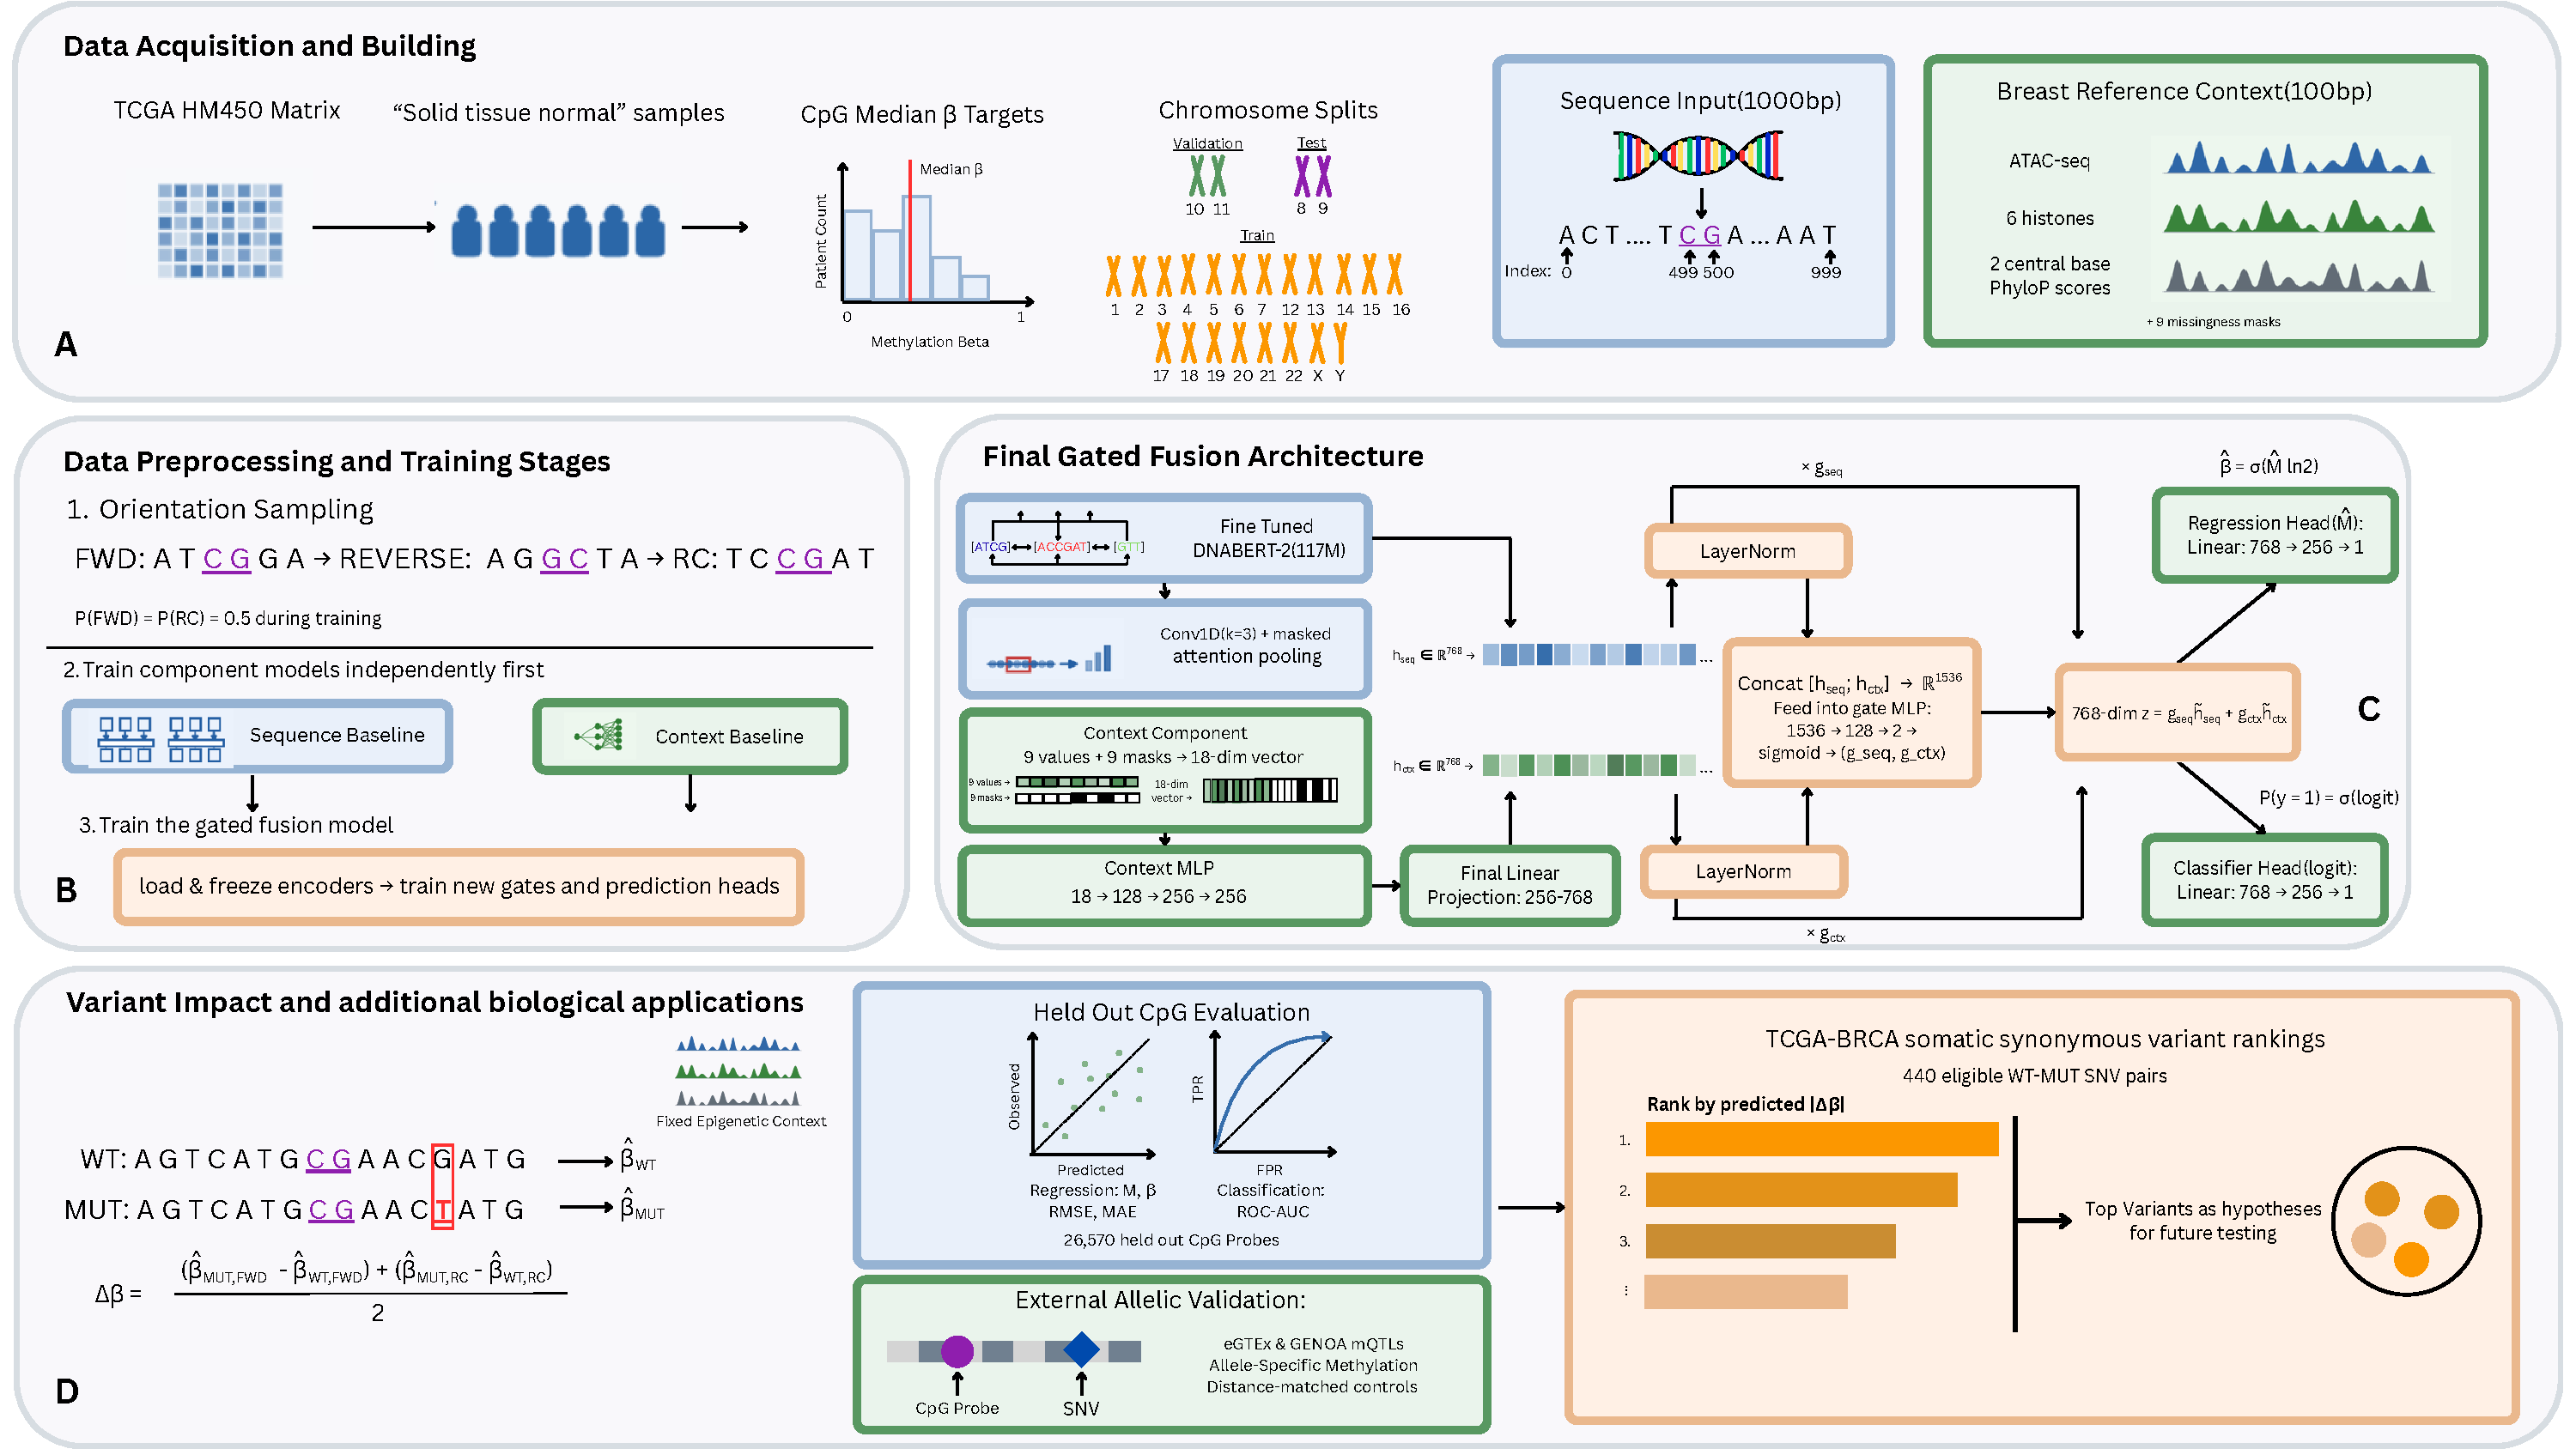
\includegraphics[width=\textwidth]{fig1.pdf}
\caption{\textbf{SilentMethyl separates baseline methylation prediction from variant-effect evaluation.}
\textbf{a}, Cohort-median methylation targets, chromosome splits and model inputs.
\textbf{b}, Sequence and context models are trained separately, then frozen for fusion training.
\textbf{c}, Normalized sequence and context representations are combined through learned gates.
\textbf{d}, Baseline testing, external variant evaluation and variant prioritization. WT and MUT use the same context, and difference predictions are averaged across forward and reverse-complement orientations.}
\label{fig:silentmethyl_workflow}
\end{figure*}

\subsection{Epigenomic context shapes prediction gains and cross-tissue generalization}
Stratified biological and epigenomic groups showed certain patterns in sequence-to-fusion improvement. Fusion reduced beta MAE across every GENCODE region, CpG island status, ATAC-seq, and H3K27ac stratum. Large relative improvements came from the highest ATAC-seq and H3K27ac quartiles, where error decreased by 22.4\% and 22.9\%, respectively (Fig.~\ref{fig:performance}g).

These results show that the benefits of incorporating reference context vary across regulatory environments. Reference information may have provided useful complementary evidence at areas of high ATAC-seq and H3K27ac signal, while the sequence model may have struggled more in making accurate predictions there.

CpG shores showed a larger absolute error improvement from fusion than islands, but their sequence-only error was also higher. Relative reductions were 17.3\% at shores and 18.4\% at islands. The highest H3K27me3 quartile had the smallest relative improvement among the tested groups, at 10.3\%, compared with 23.9\% in the lowest quartile. These results show that higher sequence-only error does not always lead to a larger improvement from fusion. 

To evaluate multi-tissue performance, we trained an additional model across colon, kidney, and lung, while excluding breast data during training and model checkpoint selection. Each probe was assigned to a single tissue to prevent conflicting methylation targets across tissues. On the same 26,570 held-out chr8--9 CpGs, the breast held-out model achieved $\beta$ MAE 0.0978 and ROC-AUC 0.9693. Breast-excluded MAE was 0.0063 higher than the three seed breast fusion mean, while sequence only MAE was 0.0013 higher than its single-tissue counterpart. 

Predictions were the most accurate at probes with similar methylation across different tissues. The beta MAE of breast-excluded sequence model predictions ranged from 0.045 in the lowest 10\% of cross-tissue variance to 0.197 in the highest (Fig.~\ref{fig:performance}e). Prediction error was correlated with cross-tissue methylation variance ($\rho=0.488$), even after controlling for mean methylation (partial $\rho=0.475$). The worst prediction decile contained more CpG shores than the remaining probes (34.8\% vs. 24.2\%), and fewer CpG islands (21.1\% vs. 31.0\%). The most inaccurate probes also had higher H3K4me1/H3K27me3 and lower ATAC-seq signal.

These results show that transfer is more inaccurate at CpGs with larger methylation variance across tissues, but this does not imply that chromatin or DNA sequence alone explain tissue differences. In this analysis, it should also be noted that the breast-held-out model only used one training seed against the mean MAE of three distinct breast only models. 

\begin{figure*}[t]
\centering
\IfFileExists{\figperformance.pdf}{\includegraphics[width=\textwidth]{\figperformance.pdf}}{\figureplan{prediction and transfer}{a Model accuracy\quad c Calibration\\e Repeated splits\quad f Relative fusion gain}}
\caption{\textbf{Context improves methylation prediction, while tissue variance limits prediction transfer.}
\textbf{a},\,\textbf{b}, $\beta$ MAE and ROC-AUC on 26,570 held-out CpGs on chromosomes 8--9. Bars show means across seeds 42--44, and error bars show variation among seeds. The two composition and k-mer ridge baselines do not need random seeding. Panel \textbf{b} starts at chance (0.5).
\textbf{c}, Predicted versus observed $\beta$ for fusion at seed 42. The dashed line is $y=x$.
\textbf{d}, $\beta$ MAE across ten equal-width groups of observed methylation.
\textbf{e}, Breast test error for models trained on colon, kidney and lung, grouped into deciles of cross-tissue methylation variance. Includes 26,558 CpGs with methylation measurements across all four tissues.
\textbf{f}, Sequence and fusion MAE for each chromosome split at seed 42.
\textbf{g}, Percentage reduction in MAE from sequence alone to fusion, grouped by chromatin-signal quartile and CpG-island class. Intervals and per-seed results are in Source Data. }
\label{fig:performance}

\end{figure*}

\subsection{Predicted local variant effects show modest concordance with independent allele-associated methylation evidence}
To externally validate SilentMethyl's variant effect predictions, we tested the breast-trained models on eGTEx breast and GENOA African American whole-blood cohorts. These sets contained 76,893 and 66,495 variant--CpG pairs, respectively. Across the 42,866 selected GENOA pairs that did not create or destroy a CpG, 4,037 reached genome-wide significance (Fig.~\ref{fig:external}a).

For the following signed analyses, we used 418 significant eGTEx pairs and 4,037 significant GENOA pairs while excluding variants that created or destroyed a CpG. Fusion achieved signed Spearman correlation 0.236 (0.098--0.392) in eGTEx and 0.149 (0.112--0.185) in GENOA. Direction agreement was 59.6\% (54.2--65.1\%) and 55.6\% (53.8--57.2\%), respectively (Fig.~\ref{fig:external}b,\,c). These results show modest agreement between predicted and measured methylation changes. However, because tissue, ancestry and cohort design all vary in this analysis, we cannot attribute differences between eGTEx and GENOA specifically to tissue matching or ancestry. Predicted and measured effects also use different scales, so these tests do not establish the accuracy of predicted effect magnitudes.

In GENOA, pairs with $p>0.5$ showed almost no signed correlation ($\rho=-0.0006$) and direction agreement near random chance (49.8\%). Stronger associations showed clearer correspondence (Fig.~\ref{fig:external}f). Direction agreement was higher for variants within 50 bp of the target CpG (56.4\%) than for those more than 400 bp away (50.5\%).

We also used a smaller positive control set of 81 breast mQTL associations from 70 variants. On this set, signed predictions separated positive from negative observed slopes with directional AUROC 0.863 (0.772--0.941). However, predicted effect magnitudes had weak consistency with measured effect magnitudes (Spearman $\rho=0.247$, 95\% confidence interval 0.020--0.442). In a matched analysis, predicted effect magnitudes only separated 35 significant mQTLs from controls with AUROC 0.505 (0.374--0.641). Therefore, the model was capable of ranking the direction of effects, but larger predicted changes did not clearly separate significant mQTLs from controls (Supplementary Fig.~S2).

Allele-specific methylation (ASM) acts as an additional source of external validation on predicted WT--MUT differences, by measuring methylation on two separate alleles in heterozygous samples. In the Do--Tycko test, we averaged model predicted changes across scored CpGs in each SNP's differentially methylated region (DMR) and compared this average with the lab-measured allelic difference. We used 722 SNPs, including 328 with positive measured effects. Confidence intervals were constructed by resampling 179 genomic blocks.

Fusion achieved direction agreement 0.590 (0.550--0.630), signed Spearman correlation 0.241 (0.180--0.299), and directional AUROC 0.628 (0.584--0.669). The sequence-only model scored slightly higher than fusion on all three metrics, but there was no clear advantage (Fig.~\ref{fig:external}g).

Fusion also separated significant ASMs from controls in two independent datasets. Fusion AUROC was 0.5625 (0.533--0.593) in Rosenski--Dor--Kaplan and 0.5419 (0.508--0.580) in Do--Tycko, compared with sequence-only values of 0.5736 and 0.5432. Distance alone performed near random chance in both datasets, suggesting that the sequence and fusion models had the ability to separate ASMs from controls beyond variant--CpG distance alone. The datasets used different controls, so AUROCs should not be compared between them. The breast-only ASM analysis included just 53 SNPs and showed no clear improvement over chance, so ASM validation for accurate direction prediction specifically in breast tissue is limited.

In a follow-up analysis, restricting absolute measured differences to $|\Delta\beta_{\mathrm{observed}}|\geq0.2$ only slightly increased direction agreement from 0.5900 to 0.6055. Larger ASM differences may reflect other linked variants instead of stronger effects from the target SNP alone, which could explain the minimal increase. In summary, ASM provides an indirect external test of single-variant predictions while extending evaluation beyond HM450 positions.

\subsection{Variant-CpG distance accounts for part of apparent variant discrimination}
Variant--CpG distance acted as a major confound in GENOA benchmark performance, since significant pairs were typically closer together than control pairs. Distance alone separated significant associations from nonsignificant controls with AUROC 0.595 (0.582--0.610), close to fusion's AUROC of 0.600 (0.586--0.615).  This means a model could appear to identify methylation-associated variants simply by predicting larger effects for variants closer to their paired probe.

After matching significant and control pairs by distance, fusion achieved AUROC 0.556 (0.539--0.572), while the $k$-mer ridge model reached 0.5063 (0.4930--0.5191; Fig.~\ref{fig:external}d). This means that fusion retained some predictive information beyond variant--CpG distance and sequence composition to identify associated variants. However, the performance drop after distance-based matching shows that CpG--variant distance differences between associated and control pairs had a large contribution to the original results.

Retrained CpGenie and DeepCpG models also showed similar performance on external validation. Fusion exceeded DeepCpG by 0.019 AUROC (0.005--0.033) on the same distance-matched GENOA pairs. Its difference from CpGenie was smaller, at 0.005 ($-0.013$--0.021), with no significant advantage. Therefore, more accurate baseline methylation prediction did not always lead to better separation of significant mQTLs from controls.

\begin{figure*}[t]
\centering
\IfFileExists{\figexternal.pdf}{\includegraphics[width=\textwidth]{\figexternal.pdf}}{\figureplan{external allelic evaluation}{a Association landscape\quad b Rank agreement\\d Distance controls\quad g ASM validation}}
\caption{\textbf{External data support modest agreement with predicted variant effects.}
\textbf{a}, Measured effects and significance for 42,866 held-out GENOA pairs that do not create or destroy a CpG. Genome-wide significant pairs are colored by whether fusion predicts the correct direction. Predictions in \textbf{a}--\textbf{c} are averaged across seeds 42--44.
\textbf{b},\,\textbf{c}, Predicted and measured effect rank correlations in GENOA and eGTEx.  Shaded bands use its 95\% confidence limits from 500 resamples of 1-Mb blocks.
\textbf{d}, AUROC before and after distance matching, including a distance-only control.
\textbf{e}, AUROC across variant--CpG distance groups.
\textbf{f}, Fusion signed correlation and direction agreement across GENOA significance groups.
\textbf{g}, ASM results. Different colors show improvement from random chance. Shaded intervals in \textbf{e} and \textbf{f} use genomic-block resampling. Full intervals and sample sizes are in Source Data and Supplementary Table~S2.}
\label{fig:external}
\end{figure*}

\subsection{Epigenomic context influences predicted variant effects without improving external concordance}
Although fusion improved single-probe methylation prediction, it performed similarly to the sequence-only model in external variant evaluations. On the same GENOA pairs, fusion-minus-sequence differences were $-0.0010$ ($-0.0078$--0.0051) for signed Spearman correlation, 0.0017 ($-0.0050$--0.0079) for direction agreement, and $-0.0023$ ($-0.0058$--0.0010) for distance-binned AUROC. Since all confidence intervals contained zero, fusion showed no significant improvement over sequence alone in this analysis.

To understand how context impacted variant effect predictions, we separated changes in sequence representation from changes in fusion gates. Even though REF and ALT use the same reference context, their gate weights can differ because they are dependent on sequence as well. After the REF prediction, the REF sequence representation was replaced with the ALT one, while preserving the REF fusion gate weights. We then replaced the sequence gate and finally the context gate with their ALT versions. The fixed fusion regression head produced a prediction at each step. The three prediction changes add up to the full REF-to-ALT effect (Fig.~\ref{fig:context}a).

The three stages reproduced the full predicted effect within $3.2 \times10^{-7}$ across 143,388 pairs. The variance of the combined gate contributions was 18.7\% of total predicted effect variance in GENOA and 19.5\% in eGTEx. Changes in the sequence gate accounted for more variance than the context gate, whose variance was approximately 6\% of the total. Note that the components are correlated, so these variance percentages do not add up to 100\%. The breakdown depends on the order of changes and does not measure the separate biological effects of sequence and context.

Although gate changes affected predictions, they added little agreement with measured variant effects. In this particular analysis, we used a broader set of scored pairs than the significant mQTLs used in the earlier signed validation. Across GENOA, the predicted change from introducing the variant in sequence while keeping gates fixed had a signed correlation of 0.0699 with measured effects, compared with 0.0707 for full fusion. After controlling for the sequence component, the combined gate contribution had small partial correlations of 0.0152 (0.0066--0.0247) in GENOA and 0.0091 (0.0017--0.0160) in eGTEx. The model also tended to give a larger proportion of gate weight to sequence at probes with higher predicted methylation (Fig.~\ref{fig:context}b). These results show how context can change predicted variant effects without clearly improving their accuracy on external validation data.

We also tested how predictions changed when reference context was shuffled between probes or replaced with feature medians. On held-out eGTEx breast pairs, context shuffling changed baseline methylation predictions more than variant effects, with normalized changes of 0.5260 and 0.2266 (Fig.~\ref{fig:context}c). Median replacement showed the same pattern, at 0.3530 and 0.1860 (Supplementary Table~S3). Baseline predictions were more strongly correlated with their original values than variant effects after median replacement (Supplementary Table~S3).  Additional analyses of prediction disagreement and DNA motifs are reported in the Supplements (Figs.~S4 and~S5).

\begin{figure*}[t]
\centering
\IfFileExists{\figcontext.pdf}{\includegraphics[width=\textwidth]{\figcontext.pdf}}{\figureplan{context mechanism}{a Paired model differences\quad b Counterfactual paths\\c Variance and partial correlation\quad d Context perturbation}}
\caption{\textbf{Context and gate changes affect predicted methylation effects.}
\textbf{a}, The sequence representation, sequence gate and context gate are changed from REF to ALT one at a time. The three prediction changes add up to the full variant effect.
\textbf{b}, Sequence gate share versus predicted reference methylation for 76,893 eGTEx pairs. The orange curve represents median gate shares.
\textbf{c}, Predictions with original versus shuffled context for methylation levels (left) and variant effects (right). Both use the $M$ scale, and dashed lines show $y=x$.}
\label{fig:context}
\end{figure*} 

\subsection{SilentMethyl prioritizes variants for targeted experimental follow-up}
Having shown the consistency of SilentMethyl's ranked responses with external validation datasets, we then used the fusion model as a prioritization engine for 440 unique synonymous variants. Variants were ranked by the absolute predicted beta change using the fusion model at seed 42. 

Here, we use our TCGA dataset's top synonymous variant as an example of how an observed somatic change can be transformed into a biological hypothesis. chr8:g.70148394G$>$A in \textit{NCOA2} is a synonymous GGC$>$GGT substitution on transcript ENST00000452400.7. The variant is 9 bp from probe cg20699548 and located in the Gene Body. The probe cg20699548 is in an OpenSea CpG and is in the 4th quartile for ATAC-seq and 3rd quartile for H3K27ac signal compared to train data. Here, our fusion model predicted a large hypomethylating shift of $\Delta\widehat\beta=-0.1539$ (Fig.~\ref{fig:candidates}a). This variant also removes a nearby CpG, but leaves the target CpG intact.

The \textit{NCOA2} candidate also had an extreme $|\Delta\widehat\beta|$ when compared with a group of similar synonymous variants. Its absolute predicted response exceeded those of all 66 variants selected for the matched-background comparison, all of which also destroy a non-target CpG (Fig.~\ref{fig:candidates}b). This example shows how SilentMethyl can prioritize single-nucleotide variants against background mutations using predicted methylation differences.

Prioritized variants and associated genes can be investigated further to develop testable hypotheses. \textit{NCOA2} encodes a nuclear receptor coactivator, and previous work reported increased expression of the gene in some breast tumors and reduced breast cancer growth after NCOA2 depletion \cite{cai2019ncoa2}. Previous literature does not directly support a causal effect between chr8:g.70148394G$>$A and increased NCOA2 activation, but our model predicts substantial demethylation at cg20699548 due to this variant. This supports the hypothesis that chr8:g.70148394G$>$A may alter regulation in \textit{NCOA2} due to the demethylation of cg20699548. Future experiments could measure the causal methylation change due to this variant and assess how it affects \textit{NCOA2} expression and breast cancer behavior.

While SilentMethyl's prioritization engine focused on somatic synonymous variants, our framework extends to any kind of single nucleotide variant. This can simply be done by modifying any base pair in the mutated sequence from the wild type sequence while context remains fixed, regardless if the change is synonymous or not. Then, WT-MUT model differences can be calculated and ranked. As an example, we evaluated a group of studied nonsynonymous SNVs in breast cancer-related genes. The two highest-ranked variants were both located in \textit{STK11}, a gene known to be associated with hereditary breast cancer risk in Peutz--Jeghers syndrome \cite{lipsa2019stk11}.

The highest predicted variant, rs2145420809, produced a predicted shift of $\Delta\widehat\beta = 0.0890$ at probe cg16601904, being immediately adjacent to its probe. This mutation converted an encoded asparagine into a serine and is in the gene body. Its corresponding CpG, cg16601904, is located at a CpG shelf and is in the 1st quartile of ATAC-seq and 3rd quartile for H3K27ac signal. The next highest predicted mutation was rs148928808, which had a change of $\Delta\widehat\beta = -0.0520$ at probe cg08681293, despite being 205 bp downstream of the CpG. This mutation converted a tyrosine into a stop codon, removes another non-target CpG, and is in the gene body as well. Its corresponding CpG, cg08681293, is a CpG shore and in the 3rd quartile of ATAC-seq and 3rd quartile of H3K27ac signal. Both variants are on transcript NM\_000455.5 (Fig.~\ref{fig:candidates}c). Unlike the seed-42 \textit{NCOA2} output, both \textit{STK11} values are predicted means over seeds 42--44.

While biological assessment of rs2145420809 is still uncertain, rs148928808 is a known pathogenic variant associated with hereditary cancer-predisposing syndrome and Peutz-Jeghers syndrome. However, SilentMethyl's difference estimates indicate large methylation shifts at both probes due to their variants. This analysis shows how SilentMethyl can evaluate clinical variants and generate hypotheses that prioritize variants on the basis of predicted WT--MUT methylation differences. Both target probes are contained within a training split, so they are primarily made to demonstrate how the model can select non-synonymous variants within a learned background, not to provide independent validation. The established consequences of a truncating variant do not prove that its predicted methylation response occurs experimentally.

This was tested more broadly using GWAS Catalog annotations. On associated pairs, labeled and unlabeled variants were matched by distance and allele frequency. The GWAS fraction among the top 5\% of predicted effects was 0.510 (0.271--0.679) in eGTEx and 0.561 (0.402--0.728) in GENOA, without a clear difference over matched null (Fig.~\ref{fig:candidates}d). Variants with larger predicted methylation effect magnitude were not clearly more likely to have GWAS annotations after matching.

\begin{figure*}[t]
\centering
\IfFileExists{\figcandidates.pdf}{\includegraphics[width=\textwidth]{\figcandidates.pdf}}{\figureplan{variant prioritization}{a NCOA2 locus\quad b Matched background\\c STK11 examples\quad d GWAS enrichment control}}
\caption{\textbf{Predicted methylation effects help prioritize variants for testing.}
\textbf{a}, The \textit{NCOA2} candidate and held-out probe cg20699548.
\textbf{b}, The candidate's absolute predicted change is greater than those of all 66 matched synonymous variants. Predictions used fusion at seed 42.
\textbf{c}, Example of two \textit{STK11} nonsynonymous variants. Both are located in training chromosomes. 
\textbf{d}, Proportion of GWAS listed variants among the top 5\% of absolute predicted effects after distance and allele-frequency matching. Error bars show 95\% confidence intervals from resampling 1-Mb blocks.
}
\label{fig:candidates}
\end{figure*}

\section{Discussion}
SilentMethyl establishes a unified framework for two complementary tasks: predicting baseline CpG methylation and estimating how that methylation state responds to single-nucleotide variants. Across held-out chromosomes, the fusion model consistently predicted methylation more accurately than sequence alone, context alone, and retrained published models. In addition, fusion improvement over sequence alone was observed across multiple held-out chromosome splits. However, fusion did not clearly improve variant-effect prediction over sequence alone. This shows why baseline methylation estimates and variant effect prediction need to be evaluated separately.  

The contribution of epigenomic context in baseline prediction varied across regulatory environments. Larger improvements found at high ATAC and H3K27ac signal suggest that reference context is especially helpful in active regulatory regions \cite{jones2012functions,schubeler2015function,encode2012integrated}. Cross-tissue predictions were less accurate at CpGs whose methylation varied more across tissues. This identifies high tissue-variance CpGs as places where tissue-specific data or better target-matched epigenomic data could help. 

In SilentMethyl, variant-response predictions can also be evaluated independently of baseline methylation performance. External mQTL and ASM data showed modest concordance with predicted directions and rankings. These external validation tests show that the model captures some allele-associated methylation differences. However, the accuracy of predicted effect magnitudes and causal methylation changes are not directly established. These results support variant ranking based on predicted difference magnitude for future investigation. 

Accounting for variant--CpG distance was important when evaluating variant effect predictions. When used to separate significant mQTLs from controls in GENOA, distance alone performed almost as well as the fusion model. After matching variant--CpG pairs by distance, the model's discrimination decreased but was still modestly above random chance. This suggests that the model predictions contained learned information beyond distance alone, and distance differences between significant mQTLs and controls contributed to the original performance. 

The gate and context perturbation analyses explain the different roles reference context has in baseline prediction and variant effects. Although both alleles use the same reference context, fusion gates can change due to sequence differences. However, these gate changes had little agreement with measured effects. Shuffling or replacing reference context changed both single-probe methylation predictions and variant effect estimates. Overall, these tests demonstrate the role context has on direct model outputs, but do not show that context improves variant-effect prediction accuracy.    

The \textit{NCOA2} analysis demonstrates how these predictions can be translated into a specific biological hypothesis. This hypothesis could be tested by introducing the \textit{NCOA2} variant and measuring methylation at cg20699548. The \textit{STK11} analysis further expands the scope of the framework beyond synonymous variants. The pathogenic stop-gain variant has an established coding consequence, but its predicted methylation effect is still a separate hypothesis. However, neither case has been experimentally verified. The \textit{STK11} examples also use training probes.

Several limitations define the current scope of these findings. Methylation targets were taken from cohort medians of 97 TCGA solid-tissue-normal breast samples collected adjacent to tumors and may therefore retain field effects or cell-composition heterogeneity \cite{tcga2012breast,teschendorff2016field}. The epigenomic context was derived from reference tracks from primary breast epithelium rather than individual samples, and HM450 measurements cover only a subset of genomic CpGs. The additional chromosome splits do not replace validation in independent breast cohorts. In addition, external mQTL benchmarks only test germline variants and do not directly validate somatic candidates. Predictions also only consider the local input window, and the current synonymous candidate rankings still need to be checked across training seeds.  Future work should focus on independent tissue-matched validation, more probe coverage, and direct experimental testing of high priority variants to establish their methylation effects and impacts on gene regulation.

Overall, SilentMethyl provides a framework for prioritizing variants with possible local methylation effects, while the magnitude of these effects and their impact on gene regulation still need experimental validation.

\section*{Conflicts of interest}
The authors declare no conflicts of interest. 

\section*{Data and code availability}
Code, run instructions, and Supplementary Data are available at \url{https://github.com/ilikecheezits/SilentMethyl}. The repository contains data behind each figure panel, analysis summaries and file checksums. The 440 ranked TCGA BRCA variants, positive and matched mQTL analyses, model predictions over seeds, and context splits can be reproduced through the reproducibility guide. Primary sources are the GDC, eGTEx, GENOA, ENCODE, GENCODE, UCSC, and the HM450 annotation resource \cite{grossman2016gdc,oliva2023mqtl,shang2023genoa,encode2012integrated,frankish2021gencode,kent2002ucsc,zhou2017infinium}.
Details on data sources and file checksums are provided in the repository's reproduction guide.

\IfFileExists{references.bib}{%
  {\small
  \setlength{\bibsep}{1pt plus 0.2ex}
  \bibliographystyle{unsrtnat}
  \bibliography{references}}
}{%
  {\small\noindent\textit{\texttt{references.bib} was not available when this
  draft was built, so citation keys are shown in place of formatted references.
  Building alongside the project bibliography restores the full list. Verify all entries against the project bibliography before submission.}\par\medskip}
  {\small
  \begin{thebibliography}{99}
\setlength{\itemsep}{2pt}
\bibitem{jones2012functions} \texttt{jones2012functions}
\bibitem{schubeler2015function} \texttt{schubeler2015function}
\bibitem{angermueller2017deepcpg} \texttt{angermueller2017deepcpg}
\bibitem{zhou2015predicting} \texttt{zhou2015predicting}
\bibitem{avsec2021effective} \texttt{avsec2021effective}
\bibitem{zeng2017cpgenie} \texttt{zeng2017cpgenie}
\bibitem{zhou2022interact} \texttt{zhou2022interact}
\bibitem{li2026deepmethylation} \texttt{li2026deepmethylation}
\bibitem{liu2025methven} \texttt{liu2025methven}
\bibitem{jin2026melody} \texttt{jin2026melody} --- Jin, Wang, Qiao \emph{et al.},
  ``Decoding the sequence determinants of locus-specific DNA methylation across
  human tissues,'' \emph{Nat. Commun.} (2026), doi:10.1038/s41467-026-76744-5.
\bibitem{mallet2021rc} \texttt{mallet2021rc}
\bibitem{sauna2011understanding} \texttt{sauna2011understanding}
\bibitem{stergachis2013exonic} \texttt{stergachis2013exonic}
\bibitem{alvarez2025mlh1} \texttt{alvarez2025mlh1}
\bibitem{blackburn2016tp53} \texttt{blackburn2016tp53}
\bibitem{jankowska2022adamts13} \texttt{jankowska2022adamts13}
\bibitem{cai2019ncoa2} \texttt{cai2019ncoa2}
\bibitem{lipsa2019stk11} \texttt{lipsa2019stk11}
\bibitem{encode2012integrated} \texttt{encode2012integrated}
\bibitem{tcga2012breast} \texttt{tcga2012breast}
\bibitem{teschendorff2016field} \texttt{teschendorff2016field}
\bibitem{grossman2016gdc} \texttt{grossman2016gdc}
\bibitem{du2010betamvalue} \texttt{du2010betamvalue}
\bibitem{zhou2017infinium} \texttt{zhou2017infinium}
\bibitem{chen2013crossreactive} \texttt{chen2013crossreactive}
\bibitem{zhou2024dnabert2} \texttt{zhou2024dnabert2}
\bibitem{frankish2021gencode} \texttt{frankish2021gencode}
\bibitem{shang2023genoa} \texttt{shang2023genoa}
\bibitem{oliva2023mqtl} \texttt{oliva2023mqtl}
\bibitem{kent2002ucsc} \texttt{kent2002ucsc}
\bibitem{camillo2024cpgpt} \texttt{camillo2024cpgpt}
\bibitem{pollard2010phylop} \texttt{pollard2010phylop}
\bibitem{loshchilov2019adamw} \texttt{loshchilov2019adamw}
\bibitem{rosenski2025asm} \texttt{rosenski2025asm}
\bibitem{do2020asm} \texttt{do2020asm}
\bibitem{rauluseviciute2024jaspar} \texttt{rauluseviciute2024jaspar}
\bibitem{cerezo2025gwas} \texttt{cerezo2025gwas}
\end{thebibliography}}
}
\end{document}